\section{Architecture}
\label{sec:arch}

\subsection{From one to two dimensions}

In a 1-D Vernier TDC the STOP edge gains $\tlsb=\ttau{1}-\ttau{2}$ on the START
edge at every stage, and an arbiter at each stage records whether STOP has
caught up. Resolving the 31 thermometer levels therefore takes 31 stages in
each line and 31 arbiters, and the conversion latency grows with the full
$31\,\ttau{1}$. The
2-D Vernier \cite{vercesi2010} generalizes the race: with START applied to a
line of $N_X$ stages of delay $\ttau{1}$ and STOP to a line of $N_Y$ stages of
delay $\ttau{2}$, an arbiter at grid position $(i,j)$ compares the edge leaving
START stage $i$ with the edge leaving STOP stage $j$ and fires when
\begin{equation}
  \dt > i\,\ttau{1} - j\,\ttau{2}.
  \label{eq:cell}
\end{equation}
Each cell therefore measures its own threshold, and $N_X+N_Y$ stages yield up
to $N_X N_Y$ distinct thresholds. Range no longer dictates line length.

\subsection{Bijective level mapping at $k=6$}

We restrict the design space to the family
$\ttau{1}=k\,\tlsb$, $\ttau{2}=(k-1)\,\tlsb$. In this family the threshold of
cell $(i,j)$ equals $(ik - j(k-1))\,\tlsb$, an exact integer multiple of the
LSB, and the mapping from thermometer level $m$ to grid cell is bijective
\cite{vercesi2010}:
\begin{equation}
  y_m = \bigl((m-1) \bmod k\bigr) + 1,
  \qquad
  x_m = \frac{m + (k-1)\,y_m}{k},
  \qquad m = 1,\dots,31.
  \label{eq:mapping}
\end{equation}
Level $m$ is exactly one SR latch, wired straight to output $Q_m$. No OR tree
or encoder sits between arbiter and output, so combining-logic skew cannot
corrupt the code. For $k=6$ the mapping spans $x_m \le 10$ and $y_m \le 6$: a
$10\times6$ logical grid, 10 START stages and 6 STOP stages for all 31 levels.

The operating point follows from two constraints. The LSB must clear the
\SI{20}{\pico\second} specification with margin for corner spread, which sets
$\tlsb=\SI{15}{\pico\second}$. The stage delays must stay inside the window
that the delay cell can actually produce under its in-grid load
(Section~\ref{sec:method}), which selects $k=6$:
$\ttau{1}=\SI{90}{\pico\second}$ and $\ttau{2}=\SI{75}{\pico\second}$. Smaller
$k$ would require $\ttau{2}$ below the achievable minimum; larger $k$ would
lengthen both lines and add area without improving resolution.

\begin{figure}[H]
\centering
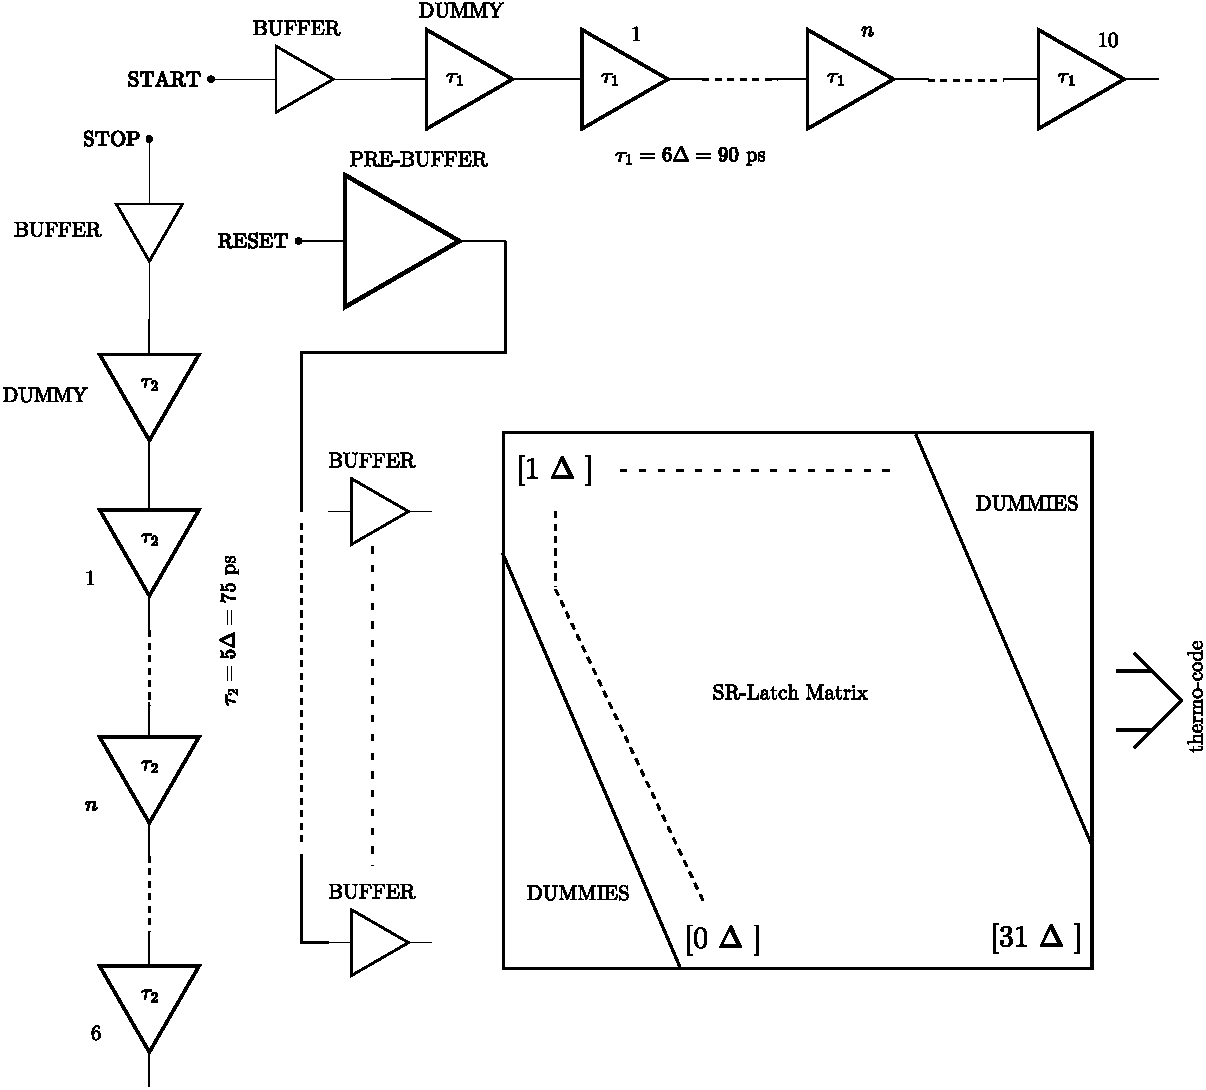
\includegraphics[width=0.82\textwidth]{figures/overview.pdf}
\caption{Top level of the converter. The START line (10 stages of $\ttau{1}$,
top) and the STOP line (6 stages of $\ttau{2}$, left) feed the SR-latch matrix.
The 31 active latches sit on the bijective map of Eq.~\eqref{eq:mapping};
dummy latches pad every tap to identical fan-out. Buffer trees distribute
START, STOP and the \SI{40}{\pico\second} RESET. The thermometer code is read
directly from the latch outputs.}
\label{fig:overview}
\end{figure}

\subsection{Fan-out equalization and reset}

Equation~\eqref{eq:cell} only holds if every stage of a line contributes the
same delay, and stage delay depends on load. In the raw $10\times6$ grid the
taps drive between one and ten latches, which would modulate the stage delays
along the line and corrupt the thresholds. We therefore pad the array with 29
dummy latches to a physically symmetric $10\times6$ arrangement: 31 active
plus 29 dummy latches give every START tap and every STOP tap the same fan-out
of ten latch inputs. The dummies are electrically identical to active latches;
only their outputs are unused. The same uniformity argument adds one extra
delay cell at the head of each line (11 and 7 cells in total), so that the
first logical stage sees the same driver as all others.

Each latch carries an asynchronous clear input. The \SI{40}{\pico\second}
RESET pulse from the testbench, widened through its own buffer tree, clears
all 60 latches before each conversion so that every conversion starts from
$Q_m=0$.
